\section{нестандартные задачи решения}
1. а) Да, так как сумма его цифр равна $1998=3\cdot666.$ б) Нет, так как последняя цифра нечётна. в) Нет, так как оно не делится на 2.\\
2. а) Нет, так как сумма его цифр равна $2\cdot239,$ что не делится на 3. б) Да, так как последняя цифра чётна. в) Нет, так как оно не делится на 3.\\
3. Раз $\text{НОД}(a,b)=a,\ b$ делится на $a,$  а поэтому  $\text{НОК}(a,b)=b.$\\
4. Раз $\text{НОК}(a,b)=a,\ a$ делится на $b,$  а поэтому  $\text{НОД}(a,b)=b.$\\
5. Всего ходящих в кружки ребят $35-10=25.$ Если сложить математиков и членов кружка <<Умелые руки>>, получим $20+11=31,$ что на $31-25=6$ больше, чем общее количество ребят, посещающих кружки. Это произошло потому, что математиков, посещающих кружок <<Умелые руки>>, мы посчитали 2 раза, значит их и было 6.\\
6. Всего ходящих в кружки ребят $37-10=27.$ Если сложить физиков и биологов, получим $19+13=32,$ что на $32-27=5$ больше, чем общее количество ребят, посещающих кружки. Это произошло потому, что физиков, посещающих кружок биологии, мы посчитали 2 раза, значит их и было 5.\\
7. Обозначим первое число буквой $x,$ тогда $x(x+2)+120=(x+4)(x+6),\ x^2+2x+120=x^2+6x+4x+24,\ 8x=96,\ x=12.$ Значит, это числа 12, 14, 16, 18.\\
8. Обозначим первое число буквой $x,$ тогда $x(x+2)+144=(x+4)(x+6),\ x^2+2x+144=x^2+6x+4x+24,\ 8x=120,\ x=15.$ Значит, это числа 15, 17, 19, 21.\\
9. Если $a$ и $b$ имеют одинаковую чётность, то оба множителя чётны и произведение должно делиться на 4, а 6 не делится. Если
$a$ и $b$ имеют разную чётность, то оба множителя нечётны и произведение должно быть нечётно, а 6 чётно. Значит, таких чисел не существует.\\
10. Если $a$ и $b$ имеют одинаковую чётность, то оба множителя чётны и произведение должно делиться на 4, а 10 не делится. Если
$a$ и $b$ имеют разную чётность, то оба множителя нечётны и произведение должно быть нечётно, а 10 чётно. Значит, таких чисел не существует.\\
11. Пусть это было число $\overline{abc}=100a+10b+c,$ тогда $100a+10b+c-a-b-c=189,\ 99a+9b=189,\ 11a+b=21.$ Если $a=1,$ то $b=10,$ что невозможно, так как это цифра. Если $a\geqslant2,$ то $11a\geqslant22>21.$ Значит, такого числа не существует и 189 получиться не могло.\\
12. Пусть это было число $\overline{abc}=100a+10b+c,$ тогда $100a+10b+c-a-b-c=180,\ 99a+9b=180,\ 11a+b=20.$ Это возможно, если $a=1,\ b=9,$ при этом цифра $c$ может быть какой угодно. Например, $190-(1+9+0)=180.$\\
13. Введём систему координат с центром в левом нижнем угле прямоугольника. Тогда диагональ --- это прямая $y=\cfrac{239}{566}x.$ Она не проходит ни через один узел сетки внутри прямоугольника, так как в таком случае и $x,$ и $y$ были бы целыми числами что невозможно, так как $x<566$ и $\text{НОД}(239,566)=1,$ поэтому домножение на $x$ не сможет сократить полностью знаменатель. Значит, диагональ пересекает по 1 разу в разных точках все вертикальные прямые $x=1,\ 2,\ \ldots 566$ и горизонтальные прямые $y=1,\ 2,\ \ldots 239,$ за исключением последней точки, правой верхней вершины прямоугольника. Последняя точка считается два раза, поэтому всего точек пересечения $566+239-1=804.$ Каждой точке пересечения можно сопоставить ту клетку, в которой диагональ находилась перед пересечением (будем считать, что мы двигаемся вправо-вверх), тогда диагональ пересекает 804 клетки.
\begin{figure}[ht!]
\center{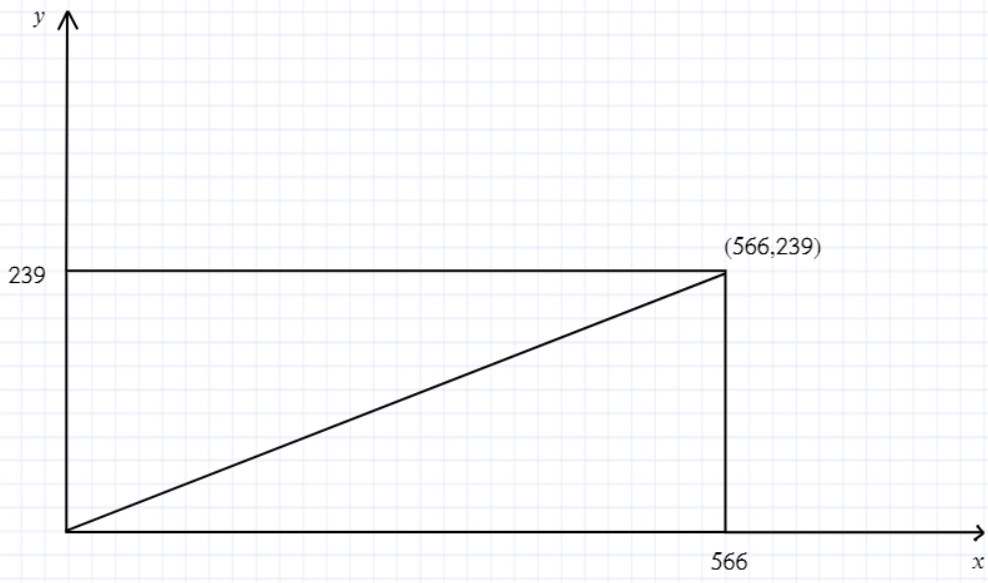
\includegraphics[scale=0.25]{566.png}}
\end{figure}\\
14. Введём систему координат с центром в левом нижнем угле прямоугольника. Тогда диагональ --- это прямая $y=\cfrac{239}{366}x.$ Она не проходит ни через один узел сетки внутри прямоугольника, так как в таком случае и $x,$ и $y$ были бы целыми числами что невозможно, так как $x<366$ и $\text{НОД}(239,366)=1,$ поэтому домножение на $x$ не сможет сократить полностью знаменатель. Значит, диагональ пересекает по 1 разу в разных точках все вертикальные прямые $x=1,\ 2,\ \ldots 366$ и горизонтальные прямые $y=1,\ 2,\ \ldots 239,$ за исключением последней точки, правой верхней вершины прямоугольника. Последняя точка считается два раза, поэтому всего точек пересечения $366+239-1=604.$ Каждой точке пересечения можно сопоставить ту клетку, в которой диагональ находилась перед пересечением (будем считать, что мы двигаемся вправо-вверх), тогда диагональ пересекает 604 клетки.
\begin{figure}[ht!]
\center{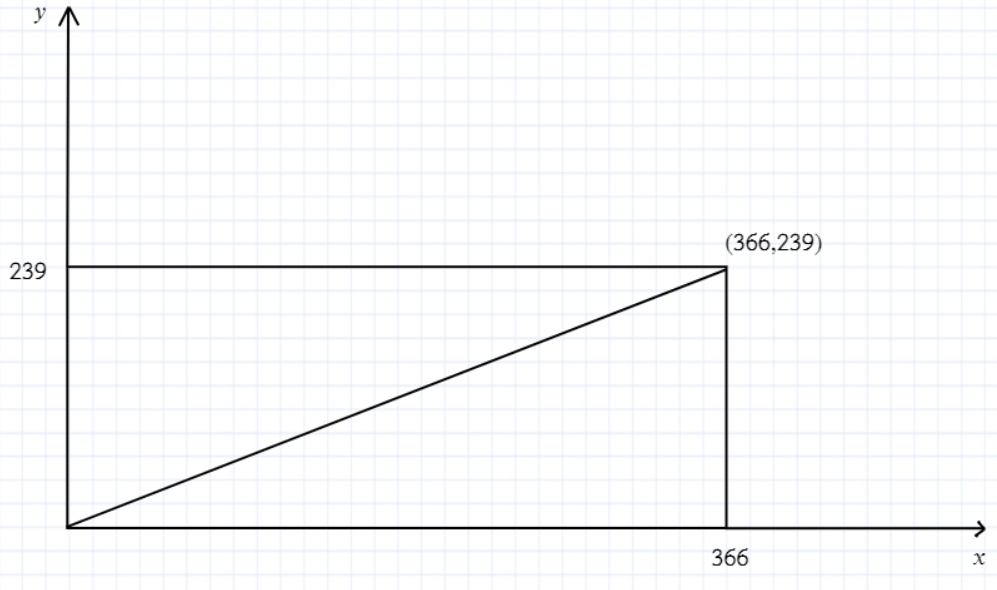
\includegraphics[scale=0.25]{5666.png}}
\end{figure}\\
15. Любые две окружности могут иметь максимум две точки пересечения. Количество способов выбрать две окружности из 9 равно $\cfrac{9\cdot8}{2}=36,$ тогда точек пересечения будет $36\cdot2=72.$\\
16. В этой последовательности на месте с номером $2k$ стоит число $k,$ а на месте с номером $2k+1$--- число $-k.$ Тогда на 366-м места стоит число $366:2=183,$ а число 366 стоит на месте $366\cdot2=732.$\\
17. В этой последовательности на месте с номером $2k$ стоит число $k,$ а на месте с номером $2k+1$--- число $-k.$ Тогда на 239-м места стоит число $-(239-1):2=-119,$ а число 239 стоит на месте $239\cdot2=478.$\\
18. Сложим числитель и знаменатель: $5k^2+7k+11+8k^2+6k+2=13k^2+13k+13=13(k^2+k+1).$ Так как сумма числителя и знаменателя делится на 13, знаменатель тоже делится на 13, а значит дробь можно сократить на 13.\\
19. Сложим числитель и знаменатель: $3k^2+7k+1+8k^2+4k+10=11k^2+11k+11=11(k^2+k+1).$ Так как сумма числителя и знаменателя делится на 11, знаменатель тоже делится на 11, а значит дробь можно сократить на 11.\\
20. Сумма возрастов игроков до удаления была равна $11\cdot22=242$ года, а после удаления стала равна $10\cdot21=210.$ Значит, удалённому игроку было $242-210=32$ года.\\
21. Сумма возрастов игроков до удаления была равна $11\cdot26=288$ лет, а после удаления стала равна $10\cdot25=250.$ Значит, удалённому игроку было $286-250=36$ лет.\\
22. Разложим число 1072 на простые множители: $1072=2^4\cdot67.$ Эти множители необходимо разбить на две группы так, чтобы произведение множителей в первой группе было больше 100 (цена книги), а во второй --- больше 6 (количество книг). Это можно сделать единственным образом: $1072=8\cdot134,$ значит книг было 8.\\
23. Разложим число 1071 на простые множители: $1071=3^2\cdot7\cdot17.$ Эти множители необходимо разбить на две группы так, чтобы произведение множителей в первой группе было больше 100 (цена книги), а во второй --- больше 5 (количество книг). Это можно сделать двумя способами: $1071=9\cdot119$ и $1071=7\cdot153.$ Значит, книг могло быть 7 или 9.\\
24. а) Пусть в первом штабеле $x$ коробок по 19кг. Тогда в нём $30-x$ коробок по 49 кг, во втором штабеле $33-x$ коробок по 19кг и $30-(33-x)=x-3$ коробки по 49 кг.
Поэтому $A=|S_1-S_2|=|19x+49(30-x)-19(33-x)-49(x-3)|=|990-60x|=30|33-2x|\geqslant30$кг, так как $|33-2x|\geqslant1.$\\
б) Пусть в первом штабеле $x$ коробок по 19кг и $y$ коробок по 49кг. Тогда во втором штабеле $33-x$ коробок по 19кг и $27-y$ коробок по 49кг. Поэтому
$A=|S_1-S_2|=|19x+49y-19(33-x)-49(27-y)|=2|19x+49y-975|.$ Если это выражение равно нулю, то $19x+49y=975,\ 19(x+y)=15(65-2y).$ Правая часть нечётна и делится на 15, числа 19 и 15 взаимно просты, значит $x+y$ может быть равно только 15 или 45 $(x+y\leqslant33+27=60<75).$ В первом случае $2y=65-19=46,\ y=23,\ x=15-23=-8,$ что невозможно. Во втором случае $2y=65-57=8,\ y=4,\ x=45-4=41>30,$ что также невозможно. Значит, $A$ не может быть равно нулю.\\
25. а) Пусть в первом штабеле $x$ коробок по 13кг. Тогда в нём $22-x$ коробок по 29 кг, во втором штабеле $25-x$ коробок по 13кг и $22-(25-x)=x-3$ коробки по 29 кг.
Поэтому $A=|S_1-S_2|=|13x+29(22-x)-13(25-x)-29(x-3)|=|400-32x|=16|25-2x|\geqslant16$кг, так как $|25-2x|\geqslant1.$\\
б) Пусть в первом штабеле $x$ коробок по 13кг и $y$ коробок по 29кг. Тогда во втором штабеле $25-x$ коробок по 13кг и $19-y$ коробок по 29кг. Поэтому
$A=|S_1-S_2|=|13x+29y-13(25-x)-29(19-y)|=2|13x+29y-438|.$ Если это выражение равно нулю, то $13x+29y=438,\ 13(x+y)=2(219-8y).$ Правая часть делится на 13, числа 2 и 13 взаимно просты, значит $219-8y$ делится на 13. Перебором остатков от деления на 13 найдём, что $y$ (при условии $0\leqslant y\leqslant19)$ может быть равно только 3 или 16. Тогда в первом случае $x=30-3=27>25,$ что невозможно. Во втором случае $x=14-16=-2,$ что также невозможно. Значит, $A$ не может быть равно нулю.\\
26. а) Да, подбором (отталкиваясь от числа 8) найдём подходящий пример.
\begin{figure}[ht!]
\center{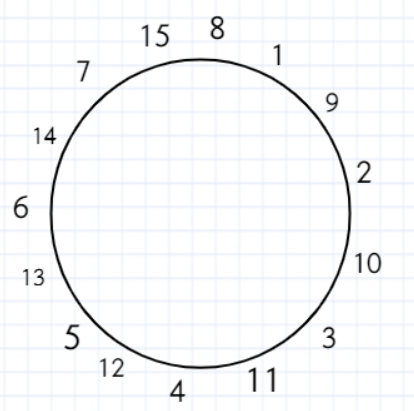
\includegraphics[scale=0.35]{krug1.png}}
\end{figure}\\
б) Нет, так как ни одно число не может стоять рядом с 8.\\
27. а) Да, подбором (отталкиваясь от числа 9) найдём подходящий пример.
\begin{figure}[ht!]
\center{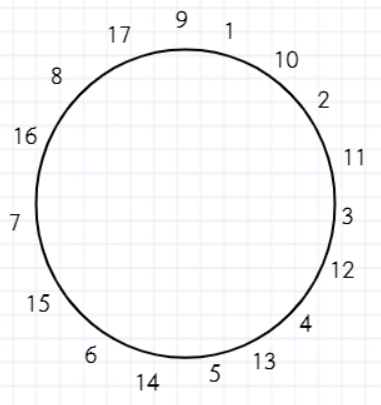
\includegraphics[scale=0.35]{krug2.png}}
\end{figure}\\
б) Нет, так как ни одно число не может стоять рядом с 9.\\
28. Число кратно трём тогда и только тогда, когда его сумма цифр делится на три. Если первые две цифры числа отличаются на 1, их сумма нечётна. Поэтому если последняя цифра числа равна 7, то сумма двух первых может быть равна 5, 11 или 17. Таких чисел 6: 237, 327, 567, 657, 897, 987. Если же последняя цифра числа равна 8, то сумма первых двух может быть равна 1, 7 или 13. Таких чисел 5: 108, 348, 438, 678, 768. Таким образом, всего {\it хороших} чисел $6+5=11.$\\
29. Число кратно трём тогда и только тогда, когда его сумма цифр делится на три. Если первые две цифры числа отличаются на 2, их сумма чётна. Поэтому если последняя цифра числа равна 6, то сумма двух первых может быть равна 6 или 12. Таких чисел 4: 246, 426, 576, 756. Если же последняя цифра числа равна 7, то сумма первых двух может быть равна 2, 8 или 14. Таких чисел 5: 207, 357, 537, 687, 867. Таким образом, всего {\it интересных} чисел $4+5=9.$\\
30. Посчитаем массу всех глыб: $50\cdot700+60\cdot1000+80\cdot1500=215000\text{ кг}=215\text{ т}.$ Будем сразу пытаться решить пункт б): $43\cdot5=215,$ значит если эти глыбы и можно погрузить на 43 грузовика, то пустого пространства ни в одном грузовике остаться не должно. Если пустого пространства не остаётся, глыб по 700кг в грузовике может быть только 5, тогда оставшиеся 1500кг занимает одна глыба по 1500кг. Понадобится $50:5=10$ грузовиков, на которые мы погрузим все глыбы по 700кг и 10 глыб по 1500кг. Остаётся ещё 60 глыб по 1000кг и $80-10=70$ глыб по 1500кг. Если пустого пространства не остаётся, глыб по 1500кг в грузовике может быть только 2, тогда оставшиеся 2000кг занимают две глыбы по 1000кг. Понадобится $60:2=30$ грузовиков, на которые мы погрузим все глыбы по 1000кг и $2\cdot30=60$ глыб по 1500кг. Таким образом, останется ещё $70-60=10$ глыб по 1500кг. Уже понятно, что в 43 грузовика все глыбы погрузить не получится, так как без пустого пространства погрузить оставшиеся глыбы невозможно. В 44 грузовика их можно погрузить следующим образом: в 3 грузовика поместить по 3 глыбы, а в последний --- одну. Тогда всего понадобится как раз $10+30+3+1=44$ грузовика.\\
31. Посчитаем массу всех глыб: $50\cdot800+60\cdot1000+60\cdot1500=190000\text{ кг}=190\text{ т}.$ Будем сразу пытаться решить пункт б): $38\cdot5=190,$ значит если эти глыбы и можно погрузить на 38 грузовиков, то пустого пространства ни в одном грузовике остаться не должно. Если пустого пространства не остаётся, глыб по 800кг в грузовике может быть только 5, тогда оставшиеся 1000кг занимает одна глыба по 1000кг. Понадобится $50:5=10$ грузовиков, на которые мы погрузим все глыбы по 800кг и 10 глыб по 1000кг. Остаётся ещё 60 глыб по 1500кг и $60-10=50$ глыб по 1000кг. Если пустого пространства не остаётся, глыб по 1500кг в грузовике может быть только 2, тогда оставшиеся 2000кг занимают две глыбы по 1000кг. Понадобится $50:2=25$ грузовиков, на которые мы погрузим все глыбы по 1000кг и $2\cdot25=50$ глыб по 1500кг. Таким образом, останется ещё $60-50=10$ глыб по 1500кг. Уже понятно, что в 38 грузовиков все глыбы погрузить не получится, так как без пустого пространства погрузить оставшиеся глыбы невозможно. В 39 грузовиков из можно погрузить следующим образом: в 3 грузовика поместить по 3 глыбы, а в последний --- одну. Тогда всего понадобится как раз $10+25+3+1=39$ грузовиков.\\
32. Пусть меньшее из чисел равно $x,$ тогда $x(x+10)-40=39x+22,\ x^2+10x-40=39x+22,\ x^2-29x-62=0,\ x^2+2x-31x-62=0,\ x(x+2)-31(x+2)=0,\ (x-31)(x+2)=0.$ Так как числа натуральные, это могут быть только 31 и $31+10=41.$\\
33. Пусть меньшее из чисел равно $x,$ тогда $x(x+10)-60=49x+22,\ x^2+10x-60=49x+22,\ x^2-39x-82=0,\ x^2+2x-41x-82=0,\ x(x+2)-41(x+2)=0,\ (x-41)(x+2)=0.$ Так как
числа натуральные, это могут быть только 41 и $41+10=51.$\\
34. Пусть изначально в каждом пакетике было $a$ шариков, а коробок было $b.$ Тогда приравняем общее количество шариков в двух случаях: $2ab=3(a-3)(b-1),\ 2ab=3ab-3a-9b+9,\ 0=ab-3a-9b+9,\ a(b-3)-9(b-3)-18=0,\ (a-9)(b-3)=18.$ Теперь необходимо разобрать все способы разложения числа 18 на два множителя, для каждого из них вычисляя общее количество шариков. Если $a-9=18,\ b-3=1,$ то $2ab=216.$ Если $a-9=9,\ b-3=2,$ то $2ab=180.$ Если $a-9=6,\ b-3=3,$ то $2ab=180.$ Если $a-9=3,\ b-3=6,$ то $2ab=216.$ Если $a-9=2,\ b-3=9,$ то $2ab=264.$ Если $a-9=1,\ b-3=18,$ то $2ab=420.$ Таким образом, наименьшее возможное количество шариков равно 180, а наибольшее --- 420.\\
35. Пусть изначально в каждом пакетике было $a$ шариков, а коробок было $b.$ Тогда приравняем общее количество шариков в двух случаях: $3ab=2(a+3)(b+1),\ 3ab=2ab+2a+6b+6,\ ab-2a-6b-6=0,\ a(b-2)-6(b-2)-18=0,\ (a-6)(b-2)=18.$ Теперь необходимо разобрать все способы разложения числа 18 на два множителя, для каждого из них вычисляя общее количество шариков. Если $a-6=18,\ b-2=1,$ то $3ab=216.$ Если $a-6=9,\ b-2=2,$ то $3ab=180.$ Если $a-6=6,\ b-2=3,$ то $3ab=180.$ Если $a-6=3,\ b-2=6,$ то $3ab=216.$ Если $a-6=2,\ b-2=9,$ то $3ab=264.$ Если $a-6=1,\ b-2=18,$ то $3ab=420.$ Таким образом, наименьшее возможное количество шариков равно 180, а наибольшее --- 420.\\
36. Максимальное количество очков, которое можно получить за один бросок, равно $20\cdot3=60.$ За 14 бросков набрать 881 очко невозможно, так как $14\cdot60=840<881.$ За 15 бросков это можно сделать следующим образом: $13\cdot60+50+51=881$ (51 очко получается как утроение 17).\\
37. Максимальное количество очков, которое можно получить за один бросок, равно $20\cdot3=60.$ За 13 бросков набрать 824 очка невозможно, так как $13\cdot60=780<824.$ За 14 бросков это можно сделать следующим образом: $12\cdot60+50+54=824$ (54 очка получается как утроение 18).\\
38. Пусть расстояние до института равно $s,$ а скорость Агаты на обратном пути равна $v.$ Тогда средняя скорость вычисляется по формуле $\cfrac{2s}{\cfrac{s}{100}+\cfrac{s}{v}}=\cfrac{2s}{\cfrac{sv+100s}{100v}}=\cfrac{200v}{v+100}.$\\
а) Приравняем это выражение к 90: $\cfrac{200v}{v+100}=90,\ 200v=90v+9000,\ 110v=9000,\ v=\cfrac{900}{11}.$ Получившийся ответ целым числом не является, значит средняя скорость за эти две поездки не может составить 90 км/ч.\\
б) Возьмём $v=60,$ тогда $\cfrac{200\cdot60}{60+100}=75.$ Значит, средняя скорость за эти две поездки может оказаться равной целому числу километров в час.\\
39. Пусть расстояние до института равно $s,$ а скорость Насти на обратном пути равна $v.$ Тогда средняя скорость вычисляется по формуле $\cfrac{2s}{\cfrac{s}{80}+\cfrac{s}{v}}=\cfrac{2s}{\cfrac{sv+80s}{80v}}=\cfrac{160v}{v+80}.$\\
а) Приравняем это выражение к 70: $\cfrac{160v}{v+80}=70,\ 160v=70v+5600,\ 90v=5600,\ v=\cfrac{560}{9}.$ Получившийся ответ целым числом не является, значит средняя скорость за эти две поездки не может составить 70 км/ч.\\
б) Возьмём $v=20,$ тогда $\cfrac{160\cdot20}{20+80}=32.$ Значит, средняя скорость за эти две поездки может оказаться равной целому числу километров в час.\\
40. Раз имеет смысл говорить о трети и о четверти учеников, количество учеников в школе делится на 3 и на 4, а значит делится и на 12. Пусть в школе учится $12x$ человек. Тогда двойки получили $12x:3+12=4x+12$ человек, а тройки --- $12x:4+18=3x+18$ человек. Раз некоторые ещё получили четвёрки, верно неравенство $4x+12+3x+18<12x,\ 7x+30<12x,\ 30<5x,\ x>6.$ Вычтем из количества двоечников количество троечников: $4x+12-(3x+18)=4x+12-3x-18=x-6>0.$ Раз получилось положительное число, двоечников больше, чем троечников.\\
41. Раз имеет смысл говорить о трети и о четверти учеников, количество учеников в школе делится на 3 и на 4, а значит делится и на 12. Пусть в школе учится $12x$ человек. Тогда двойки получили $12x:3+20=4x+20$ человек, а тройки --- $12x:4+30=3x+30$ человек. Раз некоторые ещё получили четвёрки, верно неравенство $4x+20+3x+30<12x,\ 7x+50<12x,\ 50<5x,\ x>10.$ Вычтем из количества двоечников количество троечников: $4x+20-(3x+30)=4x+20-3x-30=x-10>0.$ Раз получилось положительное число, двоечников больше, чем троечников.\\
42. а) Например, набор $\{1,\ 3,\ 4\}$ является хорошим, так как $1+3=4.$\\
б) Нет, так как $10>4+3+2.$\\
в) Например, набор $\{1,\ 9,\ 2,\ 8,\ 3,\ 7,\ 4,\ 6\}$ можно разбить на наборы $\{1,\ 9,\ 2,\ 8,\}$ и $\{3,\ 7,\ 4,\ 6\}.$ Суммы чисел в обоих наборах равны 20, при этом сами наборы являются хорошими, так как $1+9=2+8$ и $3+7=4+6.$\\
43. $(18\vee 3)\cdot3=18\cdot(3\vee3)=18\cdot1=18,$ откуда $18\vee3=18:3=6.$\\
44. а) Да, например числа 6, 7, 8, 9, 10. Наименьшее произведение равно $6\cdot7=42>40,$ а наибольшее --- $9\cdot10=90<100.$\\
б) Если расположить числа по возрастанию, то второе число равно как минимум 7, иначе произведение двух самых маленьких чисел не превосходит $6\cdot5=30<40.$ При этом пятое число равно максимум 9, иначе произведение двух самых больших чисел равно как минимум $10\cdot11=110>100.$ Но между вторым и пятым числом находятся два числа (третье и четвёртое), а между 7 и 9 только одно (8). Значит, 6 чисел быть не может.\\
45. Если число делится на 3, на 4 и на 5, то оно делится на $3\cdot4\cdot5=60,$ так как числа 3, 4 и 5 попарно взаимно просты. Всего трёхзначных чисел $999-100+1=900,$ на 60 делятся $900:60=15$ из них.\\
46. $\cfrac{x^{47}+x^{46}+\ldots+x+1}{x^{15}+x^{14}+\ldots+x+1}=\cfrac{(x-1)(x^{47}+x^{46}+\ldots+x+1)}{(x-1)(x^{15}+x^{14}+\ldots+x+1)}=$\\$
\cfrac{x^{48}+x^{47}+\cdots+x^2+x-x^{47}-x^{46}-\ldots-x-1}{x^{16}+x^{15}+x^{14}+\ldots+x-x^{15}-x^{14}-\ldots-x-1}=\cfrac{x^{48}-1}{x^{16}-1}=
\cfrac{(x^{16}-1)(x^{32}+x^{16}+1)}{x^{16}-1}=x^{32}+x^{16}+1.$\\
47. $2\#(3\#4)=2\#(2\cdot3+4)=2\#10=2\cdot2+10=14.$\\
48. Число тем меньше, чем меньше в нём цифр, поэтому наименьшее {\it счастливое} число равно 3999.\\
49. $\cfrac{n+1}{n-4}=\cfrac{n-4+5}{n-4}=1+\cfrac{5}{n-4}\leqslant1+5=6.$\\
50. $2^{30}\cdot5^7=2^{23}\cdot10^7.$ Значит, последняя ненулевая цифра этого числа равна последней ненулевой цифре числа $2^{23}.$ У степеней двойки последние цифры изменяются по следующему правилу: 2, 4, 8, 6, 2, 4, $\ldots$ Цикл имеет длину 4, а 23 даёт при делении на 4 остаток 3, значит последняя цифра будет равна 8.\\
51.
\begin{figure}[ht!]
\center{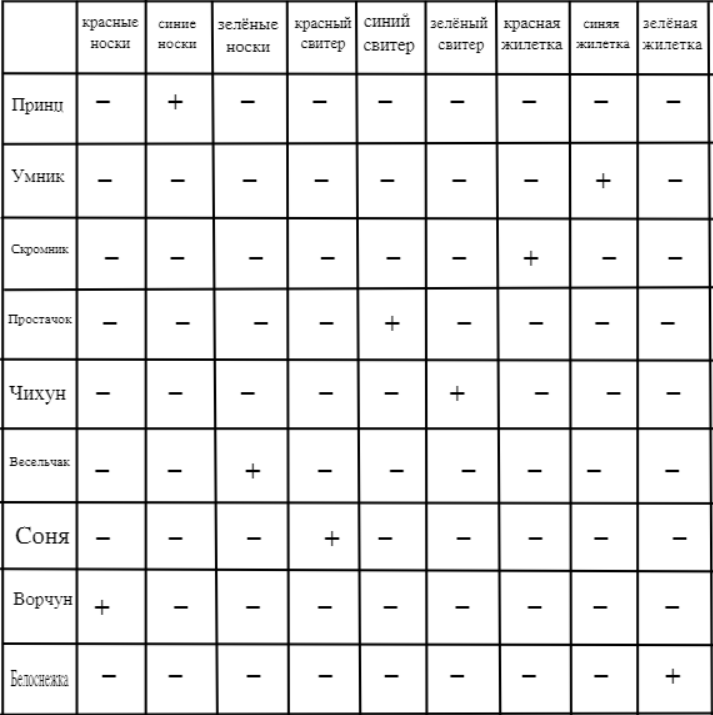
\includegraphics[scale=0.7]{pod.png}}
\end{figure}\\
Для решения этой задачи необходимо нарисовать таблицу и последовательно её заполнить. Принцу ставим $-$ во все клетки, кроме ЗЖ и СН. Умнику ставим $-$ во все клетки, кроме СН и СС. Скромнику ставим $-$ во все клетки, кроме КЖ, СС и СЖ. Простачку ставим $-$ во все клетки, кроме СС и СЖ. Чихуну и Весельчаку ставим $-$ в клетки КН, КС и КЖ. Соне ставим $-$ в КН. Весельчаку также ставим $-$ в СС и СЖ. Белоснежке ставим $+$ в ЗЖ, всем остальным в эту клетку $-$. Красные носки не могут достаться никому, кроме Ворчуна, ставим ему $+$ в эту клетку и $-$ в остальные. Зелёная жилетка досталась Белоснежке. поэтому Принц получил синие носки, ставим ему в эту клетку $+,$ всем остальным $-.$ Умнику остаётся только синяя жилетка, ставим ему в эту клетку $+,$ а всем остальным $-.$ Скромнику остаётся красная жилетка, ставим ему $+,$ а Соне $-.$ Простачку остаётся синий свитер, ставим ему $+,$ а остальным $-.$ Весельчаку остаются только зелёные носки, тогда Чихун должен получить зелёный свитер. Тогда Соне остаётся красный свитер и на этом распределение подарков окончено.\\
52. В каждой сотне цифра 4 встречается 11 раз в одном десятке (от .40 до .49) и по 1 разу во всех остальных, всего $11+9=20$ раз. Дополнительно сто цифр 4 встретятся в сотне от 400 до 499. Всего от 300 до 1100 содержится 8 сотен, а значит цифру 4 написали $8\cdot20+100=260$ раз.\\
53. Заметим, что $\cfrac{1}{k^2-1}=\cfrac{1}{(k-1)(k+1)}=\cfrac{1}{2}\left(\cfrac{1}{k-1}-\cfrac{1}{k+1}\right),$ поэтому
$\cfrac{1}{3}+\cfrac{1}{8}+\cfrac{1}{15}+\ldots+\cfrac{1}{n^2-1}=\cfrac{1}{2}\left(\cfrac{1}{1}-\cfrac{1}{3}+\cfrac{1}{2}-\cfrac{1}{4}+
\cfrac{1}{3}-\cfrac{1}{5}+\cfrac{1}{4}-\cfrac{1}{6}+\ldots+\cfrac{1}{n-2}-\cfrac{1}{n}+\cfrac{1}{n-1}-\cfrac{1}{n+1}\right)=
\cfrac{1}{2}\left(\cfrac{1}{1}+\cfrac{1}{2}-\cfrac{1}{n}-\cfrac{1}{n+1}\right)=$\\$=\cfrac{3n^2-n-2}{4n(n+1)}.$\\
54. Число $3^{4^5}=3^{2^{10}}=\left(3^{2^9}\right)^2$ является точным квадратом.\\
55. Пусть это число равно $n,$ тогда $n-2$ делится на 3 и на 23, а значит делится на 69. Поэтому минимальное значение $n$ равно $69+2=71.$\\
56. $633^{3^{72}}=633^{9^{36}}>633^{8^{36}}=633^{2^{108}}=633^{4^{54}}>632^{4^{54}}.$\\
57. $\cfrac{4n-23}{n-2}=\cfrac{4n-8-15}{n-2}=4-\cfrac{15}{n-2}.$ Для того, чтобы это число было натуральным, 15 должно делиться на $n-2.$ Если $n-2=15,$ то $n=17,$ а это число равно 3. Если $n-2=5,$ то $n=7,$ а это число равно 1. Если $n-2=3,$ то это число равно $-1$ и не является натуральным. Если $n-2=1,$ то это число равно $-11$ и не является натуральным. Если $n-2=-1,$ то $n=1,$ а это число равно 19. Таким образом, подходят только 1, 7 и 17.\\
58. Да, например так:
\begin{figure}[ht!]
\center{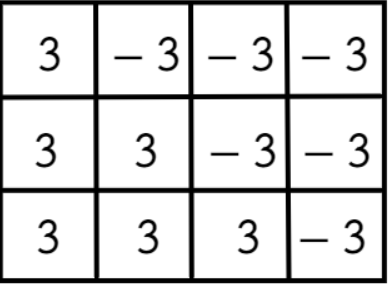
\includegraphics[scale=0.35]{tb.png}}
\end{figure}\\
59. $b^2+3b+2004=b^2+4b+4+2000-b=(b+2)^2+2000-b.$ При $b=2000$ это число равно $2002^2.$\\
60. Например, это можно сделать так:
\begin{figure}[ht!]
\center{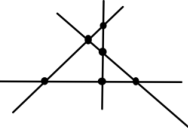
\includegraphics[scale=0.35]{aa.png}}
\end{figure}\\
61. Например, это можно сделать так:
\begin{figure}[ht!]
\center{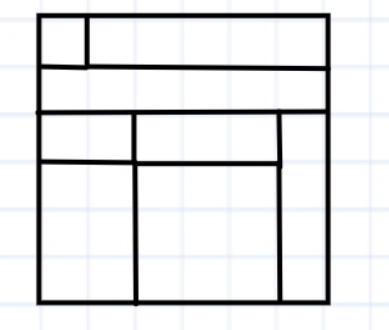
\includegraphics[scale=0.35]{aaa.png}}
\end{figure}\\
62. 3НОД(72, 80, 96)+$\frac{1}{2}$НОК(72, 80, 96)$=3\cdot8+\frac{1}{2}\cdot1440=744.$\\
63. Если число делится на 15, то оно делится на 3 и на 5. Если число делится на 5, его последняя цифра может быть только 0 или 5. Если последняя цифра равна 5, первая цифра равна $7-5=2,$ а вторая цифра должна быть такой, чтобы сумма цифр делилась на 3: 2, 5 или 8. Если последняя цифра равна 0, первая цифра равна $7-0=7,$ а вторая цифра должна быть такой, чтобы сумма цифр делилась на 3: 2, 5 или 8. Таким образом, подходят следующие числа: 225, 255, 285, 720, 750, 780.\\
64. $\left( \cfrac{1\cdot2\cdot4+2\cdot4\cdot8+\ldots+10\cdot20\cdot40}{1\cdot4\cdot5+2\cdot8\cdot10+\ldots+10\cdot40\cdot50}\right)^2=
\left( \cfrac{1\cdot2\cdot4\cdot(1+2\cdot2\cdot2+\ldots+10\cdot10\cdot10)}{1\cdot4\cdot5\cdot(1+2\cdot2\cdot2+\ldots+10\cdot10\cdot10)}\right)^2=$\\$=
\left( \cfrac{1\cdot2\cdot4}{1\cdot4\cdot5}\right)^2=\cfrac{4}{25}.$\\
65. Число 11 в любой степени заканчивается на 1. Число 9 в нечётных степенях заканчивается на 9. Последняя цифра степени двойки меняется по следующему правилу: 2, 4, 8, 6, 2, 4, ... Цикл состоит из 4 цифр, а 15 даёт остаток 3 при делении на 4, значит $2^{15}$ кончается на 8. Тогда последняя цифра числа $11^{50}+9^{35}-2^{15}$
равна $1+9-8=2.$\\
66. Пусть изначально число было равно  $\overline{ab},$ тогда $10b+a\geqslant3(10a+b),\ 10b+a\geqslant30a+3b,\ 7b\geqslant29a.$ Это неравенство может выполниться только при $a=1,\ b\in\{5,\ 6,\ 7,\ 8,\ 9\}$ или при $a=2,\ b=9.$ Всего подходит 6 чисел.\\
67. Пусть девятиклассники получили по $x$ тетрадей, а пятиклассники --- по $y.$ Тогда $12x+5y=120.$ Сумма делится на 12, как и первое слагаемое, значит второе слагаемое делится на 12, значит $y$ делится на 12. Если $y=24,$ то $x=0,$ что невозможно. Значит, $y=12,$ а тогда $x=5.$\\
68. Пусть $a\geqslant b\geqslant c$ и $a+b+c=80.$ Тогда сумма их попарных разностей равна $a-b+b-c+a-c=2(a-c).$ Наибольшее значение это выражение принимает тогда, когда разница между наибольшим и наименьшим из чисел максимальна, это достигается когда $a=77,\ b=2,\ c=1.$ Тогда это выражение равно $2\cdot(77-1)=152.$\\
69. Разложим на простые множители число 10472: $10472=2^3\cdot7\cdot11\cdot17.$ Числа 11 и 17 цифрами быть не могут, значит это делители самого числа. Тогда произведение цифр числа может быть равно 56, 28, 14, 7, 2 или 1. Небольшим перебором находим, что подходит только произведение цифр 56, само число при этом равно 187.\\
70. Пусть мы $a$ раз записали сообщение и $b$ раз удалили. В таком случае занято $500+198a-300b=2(250+99a-150b).$ Выражение $99a-150b$ всегда делится на 3, значит
$250+99a-150b$ даёт остаток 1 и таким образом не меньше 1. Тогда всего занято не менее 2 байт и полностью очистить память невозможно. Два байта можно получить, взяв $a=49,\ b=34.$\\
71. $8^7+2^{19}+4^9=2^{21}+2^{19}+2^{18}=2^{18}(2^3+2+1)=2^{18}\cdot11,$ что всегда делится на 11.\\
72. Пусть это число равно $x,$ тогда $x-1$ делится на каждое из чисел 2, 3, 4, 5, 6, а значит делится на 60. Первое делящееся на 7 число вида $60n+1$ равно 301.\\
73. Перечислим числа, при делении на которые 1000 даёт такой же остаток, как 1 или $-1:$ 3, 9, 27, 37, 111. При возведении в 1000 степень оно станет давать остаток 1 при делении на все эти числа, а значит после вычитания единицы будет на них делиться.\\
74. $k^2+(k+1)^2+(k+2)^2=k^2+k^2+2k+1+k^2+4k+4=3k^2+6k+5=3(k^2+2k+1)+2.$\\
75. Пусть $n=7k+3.$ Тогда $n^2+2n=(7k+3)^2+2(7k+3)=49k^2+42k+9+14k+6=49k^2+56k+15=7(7k^2+8k+2)+1.$\\
76. Переведём всё в копейки $15600+x$ должно делиться на 90, причём $0\leqslant x <100.$ Значит, $x$ должен делиться на 3 и на 10 (так как делится 15600), поэтому $x$ делится на 30. Из чисел 30, 60 и 90 подходит только 60, поэтому один ластик стоит $15660:90=174$ копейки или 1 рубль 74 копейки.\\
77. Разложим на простые множители: $12960=2^5\cdot3^4\cdot5.$ Чтобы число являлось квадратом целого числа, оно должно делиться только на чётные степени всех простых чисел, значит минимальное подходящее значение $T$ равно $2\cdot5=10.$\\
78. а) Пусть изначальное число равно $\overline{ab},$ тогда $10a+b+9=10b+a,\ 9a+9=9b,\ a+1=b.$ Значит, подходят числа 12, 23, 34, 45, 56, 67, 78, 89.\\
б) Пусть изначальное число равно $\overline{ab},$ тогда $10a+b-63=10b+a,\ 9a-63=9b,\ a-7=b.$ Значит, подходят числа 81, 92.\\
79. а) Самое большое простое число в этом ряду равно 157.\\
б) На 5 делятся числа от $95=5\cdot19$ до $160=5\cdot32,$ то есть $32-19+1=14$ чисел. На 25 делятся числа 100, 125 и 150, что даёт дополнительные три пятёрки. Также есть число 125, в множителях которого есть ещё одна дополнительная пятёрка. Значит, всего это произведение делится на $5^{18}.$\\
в) Двоек в этом произведении ещё больше (каждое второе число чётно), значит последние 18 цифр равны 0.\\
80. Число, кончающееся на 0, в любой степени кончается на 0. Последняя цифра степени числа, кончающегося на 7, изменяется следующим образом: 7, 9, 3, 1, 7, ...
Длина цикла равна 4, а 2008 делится на 4, значит эта степень кончается на 1. Таким образом, сумма этих чисел кончается на 1.\\
81. Раз Таня поймала окуня, Вика точно поймала щуку. Про Колю и Серёжу данных нет, так что каждый из них мог поймать плоту или леща.\\
82. Раз Вася поймал леща, плотву мог поймать только Толя. Катя с Семёно могли поймать окуня и щуку в любом порядке.\\
83. Пусть Вовочка получил $x$ пятёрок, тогда его средний балл равен $\cfrac{1+5x}{x+1}.$ Для того, чтобы средний балл стал равен 4,5, должно выполняться равенство
$\cfrac{1+5x}{x+1}=4,5,\ 1+5x=4,5x+4,5,\ 0,5x=3,5,\ x=7.$\\
84. Утверждение а) равносильно тому, что один фломастер стоит $15,86:4=3,965$ рубля. Утверждение б) равносильно тому, что один фломастер стоит $14,58:6=2,43$ рубля. Утверждение в) равносильно тому, что один фломастер стоит $18,68:8=2,335$ рубля. Так как тысячные доли рубля в расчётах участвовать не могут, верным является утверждение б).  Так как $5000:243=20$ (ост. 140), на 50 рублей можно купить 20 фломастеров.\\
85. а) Это верно, так как медиана, проведённая из прямого угла, равна половине гипотенузы.\\
б) $8^7-2^{18}=2^{21}-2^{18}=2^{18}\cdot(2^3-1)=2^{18}\cdot7,$ значит это утверждение также верно.\\
в) Это неверно, так как пары равных углов, прилежащих к равной стороне, может не найтись. Например, можно рассмотреть два равнобедренных прямоугольных треугольника (углы $90^\circ,\ 45^\circ,\ 45^\circ$), у первого из которых единице равен катет, а у второго --- гипотенуза.\\
86. Сумма всех чисел в строке равна $1+2+\ldots+37=(1+37)+(2+36)+\ldots+(18+20)+19=38\cdot18+19=703=37\cdot19.$ Сумма всех чисел, кроме последнего, делится на последнее число, а значит сумма вообще всех чисел тоже делится на последнее число. Но 703 делится только на 19, 37 и 1, а 37 и 1 написаны на первых двух местах. Значит, на последнем месте стоит число 19. На третьем месте стоит делитель числа $37+1=38,$ но числа 1 и 19 уже стоят на других местах, значит там стоит число 2.\\
87. Разложим на простые множители число $990:\ 990=2\cdot3^2\cdot5\cdot11.$ Значит $n$ должно быть как минимум 11, это значение подходит, так как до 11 есть множители 10 и 9.\\
88. Найдём самую маленькую возможную сумму семи троек: $1+2+3+\ldots+20+21=(1+21)+(2+20)+\ldots+(10+12)+11=22\cdot10+11=231.$ Теперь найдём самую большую возможную сумму семи различных чисел, не превосходящих 35: $35+34+33+32+31+30+29=224<231.$ Значит, семь троек обвести нельзя. Шесть троек обвести можно, например так:
$6+7+17=30,\ 5+8+18=31,\ 4+9+19=32,\ 3+10+20=33,\ 2+11+21=34,\ 1+12+22=35.$\\
89. Найдём самую маленькую возможную сумму девяти троек: $1+2+3+\ldots+20+27=(1+27)+(2+26)+\ldots+(15+13)+14=28\cdot13+14=378.$ Теперь найдём самую большую возможную сумму девяти различных чисел, не превосходящих 42: $42+41+40+39+38+37+36+35+34=342<378.$ Значит, девять троек обвести нельзя. Восемь троек обвести можно, например так:
$8+9+18=35,\ 7+10+19=36,\ 6+11+20=37,\ 5+12+21=38,\ 4+13+22=39,\ 3+14+23=40,\ 2+15+24=41,\ 1+16+25=42.$\\
90. НОК$(12,\ 70,\ 135) =$НОК$(2^2\cdot3,\ 2\cdot5\cdot7,\ 3^3\cdot5)=2^2\cdot3^3\cdot5\cdot7=3780.$\\
91. НОД$(2040,\ 4200)=$НОД$(2^3\cdot3\cdot5\cdot17,\ 2^3\cdot3\cdot5^2\cdot7)=2^3\cdot3\cdot5=120.$\\
92. НОК$(18,\ 30,\ 175)=$НОК$(2\cdot3^2,\ 2\cdot3\cdot5,\ 5^2\cdot7)=2\cdot3^2\cdot5^2\cdot7=3150.$\\
93. НОД$(2160,\ 10400)=$НОД$(2^4\cdot3^3\cdot5,\ 2^5\cdot5^2\cdot13)=2^4\cdot5=80.$\\
94. Число кратно 45 тогда и только тогда, когда оно кратно 5 и 9. Число кратно 5 тогда и только тогда, когда его последняя цифра 0 или 5. Значит, $b$ может быть равно 0 или 5. Число кратно 9 тогда и только тогда, когда сумма его цифр кратна 9. В первом случае $7+2+3+a+1+0=a+13$ кратно 9, тогда $a=5.$ Во втором случае
$7+2+3+a+1+5=a+18$ кратно 9, тогда $a=0$ или $a=9.$ Таким образом, подходят числа 723510, 723015 и 723915.\\
95. Число кратно 36 тогда и только тогда, когда оно кратно 4 и 9. Число кратно 4 тогда и только тогда, когда число, образованное двумя его последними цифрами, кратно 4. Значит, $b$ может быть равно 0, 4 или 8. Число кратно 9 тогда и только тогда, когда сумма его цифр кратна 9. В первом случае $6+5+a+8+0=a+19$ кратно 9, тогда $a=8.$ Во втором случае $6+5+a+8+4=a+23$ кратно 9, тогда $a=4.$ В третьем случае $6+5+a+8+8=a+27$ кратно 9, тогда $a=0$ или $a=9.$ Таким образом, подходят числа 65880, 65484, 65088 и 65988.\\
96. Число кратно 45 тогда и только тогда, когда оно кратно 5 и 9. Число кратно 5 тогда и только тогда, когда его последняя цифра 0 или 5. Значит, $b$ может быть равно 0 или 5. Число кратно 9 тогда и только тогда, когда сумма его цифр кратна 9. В первом случае $6+a+5+7+0=a+18$ кратно 9, тогда $a=0$ или $a=9.$ Во втором случае $6+5+a+7+5=a+23$ кратно 9, тогда $a=4.$ Таким образом, подходят числа 60570, 69570 и 64575.\\
97. Число кратно 36 тогда и только тогда, когда оно кратно 4 и 9. Число кратно 4 тогда и только тогда, когда число, образованное двумя его последними цифрами, кратно 4. Значит, $b$ может быть равно 0, 4 или 8.Число кратно 9 тогда и только тогда, когда сумма его цифр кратна 9. В первом случае $8+a+5+6+0=a+19$ кратно 9, тогда $a=8.$ Во втором случае $8+a+5+6+4=a+23$ кратно 9, тогда $a=4.$ В третьем случае $8+a+5+6+8=a+27$ кратно 9, тогда $a=0$ или $a=9.$ Таким образом, подходят числа 88560, 84564, 80568 и 89568.\\
98. Число $2x-20=2\cdot(x+5)-30$ кратно $x+5$ тогда и только тогда, когда 30 кратно $x+5.$ Так как число $x$ является натуральным, возможны случаи: $x+5=6,\ x=1,$ или $x+5=10,\ x=5,$ или $x+5=15,\ x=10,$ или $x+5=30,\ x=25.$\\
99. Число $k+11=k+13-2$ кратно $k+13$ тогда и только тогда, когда 2 кратно $k+13.$ Так как число $k$ является целым, возможны случаи: $k+13=2,\ k=-11,$ или $k+13=1,\ k=-12,$ или $k+13=-1,\ k=-14,$ или $k+13=-2,\ k=-15.$\\
100. Число $3x+7=3\cdot(x-2)+13$ кратно $x-2$ тогда и только тогда, когда 13 кратно $x-2.$ Так как число $x$ является натуральным, возможны случаи: $x-2=-1,\ x=1,\ x-2=1,\ x=3$ или $x-2=13,\ x=15.$\\
101. Число $2k-1=2\cdot(k+3)-7$ кратно $k+3$ тогда и только тогда, когда 7 кратно $k+3.$ Так как число $k$ является целым, возможны случаи: $k+3=7,\ k=4,$ или $k+3=1,\ k=-2,$ или $k+3=-1,\ k=-4,$ или $k+3=-7,\ k=-10.$\\
102. а) Да, $888:3=296.$\\
б) Нет, нечётное число не может делиться на чётное.\\
103. Пусть площадь их общей части равна $S,$ тогда площади областей равны $12^2-S=144-S$ и $15^2-S=225-S.$ Их разность равна $225-S-144+S=81.$\\
104. Так как знаменатели всей дробей не меньше 1, имеем соотношения $|x|\geqslant |z|, |y|\geqslant |x|,\ |z|\geqslant |y|,$ откуда
$|x|=|y|=|z|.$ Так как каждое неравенство должно обращаться в равенство, все знаменатели дробей равны 1 и $x=y=z=0.$\\
105. а) Да, 444444444 делится на 9, так как его сумма цифр $4\cdot9=36$ делится на 9.\\
б) Нет, нечётное число не может делиться на чётное.\\
106. Пусть площадь их общей части равна $S,$ тогда площади областей равны $11^2-S=121-S$ и $14^2-S=196-S.$ Их разность равна $196-S-121+S=75.$\\
107. Так как знаменатели всей дробей не меньше 1, имеем соотношения $|a|\geqslant |c|, |b|\geqslant |a|,\ |c|\geqslant |b|,$ откуда
$|a|=|b|=|c|.$ Так как каждое неравенство должно обращаться в равенство, все знаменатели дробей равны 1 и $a=b=c=0.$\\
108. $\cfrac{a^2-4b^2}{ab}=3,\ a^2-4b^2=3ab,\ a^2-3ab-4b^2=0,\ a^2+ab-4ab-4b^2=0,\ a(a+b)-4b(a+b)=0, (a+b)(a-4b)=0,\ a=4b$ (так как числа положительны). Тогда
$\cfrac{a^2+b^2}{ab}=\cfrac{a^2+16a^2}{4a^2}=\cfrac{17}{4},$ ч.т.д.\\
109. а) Попробуем подобрать пример, в котором в каждой группе по одному числу $x,\ y$ и $z.$ Они поменяются на $10x+3,\ 10y+7$ и $z.$ Тогда должно выполняться равенство $10x+3+10y+7+z=8x+8y+8z,\ 2x+2y+10=7z.$ Такие числа нетрудно подобрать, например $x=2,\ y=7, z=4.$\\
б) Пусть в первой группе $m$ чисел с суммой $x,$ во второй группе $n$ чисел с суммой $y,$ а в третьей группе числа с суммой $z.$ Тогда
$10x+3m+10y+7n+z=17x+17y+17z,\ 7x+7y+16z=3m+7n.$ Но так как все числа натуральны, $x\geqslant m$ и $y\geqslant n,$ поэтому левая часть всегда больше правой. Значит, в 17 раз сумма всех чисел увеличиться не могла.\\
110. Пусть $\cfrac{x}{2}=\cfrac{y}{3}=\cfrac{z}{4}=t,$ тогда $x=2t,\ t=3t,\ z=4t$ и $\cfrac{x+3y-z}{2x-3z}=\cfrac{2t+9t-4t}{4t-12t}=\cfrac{7t}{-8t}=-\cfrac{7}{8}.$\\
111. По количеству шариков понятно, что ребята стоят в следующем порядке: Коля, Петя, Женя, Сева. Тогда у Пети $32-21=11$ шариков, у Жени $21-13=8$ шариков, а у Севы $13-5=8$ шариков.\\
112. Пусть длинная сторона прямоугольника равна $a,$ а короткая $b,$ тогда имеем систему уравнений $\begin{cases} 3a+b=22,\\ 2a+2b=18.\end{cases}\Leftrightarrow
\begin{cases} 3a+b=22,\\ a+b=9.\end{cases}\Leftrightarrow
\begin{cases} 2a=13,\\ b=9-a.\end{cases}\Leftrightarrow
\begin{cases} a=6,5,\\ b=2,5.\end{cases}$ Тогда площадь прямоугольника равна $6,5\cdot2,5=16,25.$\\
113. $a+\cfrac{1}{b+\cfrac{1}{c}}=\cfrac{35}{11}=3\cfrac{2}{11},$ значит $a=3$ и $\cfrac{1}{b+\cfrac{1}{c}}=\cfrac{2}{11}.$ Тогда $b+\cfrac{1}{c}=\cfrac{11}{2}=5\cfrac{1}{2},$ откуда $b=5$ и $\cfrac{1}{c}=\cfrac{1}{2},$ поэтому $c=2.$ Таким образом, $abc=3\cdot5\cdot2=30.$\\
114. Заметим, что при натуральных $x$ и $y$ множители не обязательно должны быть натуральными. Рассмотрим все возможные разложения 6 на два целых множителя. Если $x-3=-6$ или $x-3=-3,$ то $x$ не является натуральным числом, что невозможно. Если $x-3=-2,$ то $x=1,$ а $y=(1-6:(-2)):2=2.$ Если $x-3=-1,$ то $x=2,$ а $y=(2-6:(-1)):2=4.$ Если $x-3=1,$ то $x=4,$ а $y=(4-6:1):2=-1,$ что невозможно. Если $x-3=2,$ то $x=5,$ а $y=(5-6:2):2=1.$ Если $x-3=3,$ то $x=6,$ а $y=(6-6:3):2=2.$ Если $x-3=6,$ то $x=9,$ а $y=(9-6:6):2=4.$ Итого $(x;y)\in\{(1;2),\ (2;4),\ (5;1),\ (6;2),\ (9;4)\}.$\\
115. Число 30303032 кончается на 2, а значит не может быть точным квадратом. Число 246801 имеет сумму цифр 21, а значит делится на 3, но не делится на 9, поэтому также не может быть точным квадратом. Число 56781234 делится на 2, но не делится на 4 (так как 34 не делится на 4), поэтому не может быть точным квадратом. Число 67812345 делится на 5, но не делится на 25 (так как 45 не делится на 25), значит и оно не может быть точным квадратом. Таким образом, точных квадратов среди приведённых чисел нет.\\
116. Пусть число имеет вид $\overline{abc}=100a+10b+c.$ Тогда $\overline{abc}-\overline{cba}=100a+10b+c-100c-10b-a=99(a-c)=198,\ a-c=2,\ a=c+2.$ Так как сумма квадратов цифр равна 101, получим равенство $b^2=101-a^2-c^2.$ Переберём все возможные значения буквы $c$ от 1 до 7. Если $c=1,$ то $a=3$ и $b^2=101-1-9=91,$ чего быть не может. Если $c=2,$ то $a=4$ и $b^2=101-4-16=81,\ b=9,$ то есть подходит число 492. Если $c=3,$ то $a=5$ и $b^2=101-9-25=67,$ чего быть не может. Если $c=4,$ то $a=6$ и $b^2=101-16-36=49,\ b=7$ то есть подходит число 674. Если $c=5,$ то $a=7$ и $b^2=101-25-49=27,$ чего быть не может. Если $c=6,$ то $a=8$ и $b^2=101-36-64=1,\ b=1,$ то есть подходит число 816. Если $c=7,$ то $a=9$ и $b^2=101-81-49=-29,$ чего быть не может. Таким образом, подходят только числа 492, 674, 816.\\
117. Обозначим искомое число буквой $x,$ тогда натуральное число $x-6$ должно делиться и на 7, и на 17. Так как числа 7 и 17 взаимно просты, наименьшее значение $x-6$ равно $7\cdot17=119,$ поэтому $x=119+6=125.$\\
118. Обозначим искомое число буквой $x,$ тогда натуральное число $x-4$ должно делиться и на 5, и на 19. Так как числа 5 и 19 взаимно просты, наименьшее значение $x-4$ равно $5\cdot19=95,$ поэтому $x=95+4=99.$\\
119. $\cfrac{1}{6}\cdot 7^{32}-(7+1)(7^2+1)(7^4+1)(7^8+1)(7^{16}+1)=\cfrac{7^{32}-(7-1)(7+1)(7^2+1)(7^4+1)(7^8+1)(7^{16}+1)}{6}=
\cfrac{7^{32}-(7^2-1)(7^2+1)(7^4+1)(7^8+1)(7^{16}+1)}{6}=\cfrac{7^{32}-(7^4-1)(7^4+1)(7^8+1)(7^{16}+1)}{6}=$\\$
\cfrac{7^{32}-(7^8-1)(7^8+1)(7^{16}+1)}{6}=\cfrac{7^{32}-(7^{16}-1)(7^{16}+1)}{6}=\cfrac{7^{32}-(7^{32}-1)}{6}=\cfrac{1}{6}.$\\
120. $\cfrac{1}{4}\cdot 5^{32}-(5+1)(5^2+1)(5^4+1)(5^8+1)(5^{16}+1)=\cfrac{5^{32}-(5-1)(5+1)(5^2+1)(5^4+1)(5^8+1)(5^{16}+1)}{4}=
\cfrac{5^{32}-(5^2-1)(5^2+1)(5^4+1)(5^8+1)(5^{16}+1)}{4}=\cfrac{5^{32}-(5^4-1)(5^4+1)(5^8+1)(5^{16}+1)}{4}=$\\$
\cfrac{5^{32}-(5^8-1)(5^8+1)(5^{16}+1)}{4}=\cfrac{5^{32}-(5^{16}-1)(5^{16}+1)}{4}=\cfrac{5^{32}-(5^{32}-1)}{4}=\cfrac{1}{4}.$\\
121. Если $2n-1>n-5>0,$ то дробь точно не может быть целой, так как является правильной. Значит, достаточно разобрать случаи $n\in\{1; 2; 3; 4; 5\}.$ При $n=1$ дробь равна $\cfrac{1-5}{2\cdot1-1}=-4,$ это значение подходит. При $n=2$ дробь равна $\cfrac{2-5}{2\cdot2-1}=-1,$ это значение тоже подходит.
При $n=3$ дробь равна $\cfrac{3-5}{2\cdot3-1}=-0,4,$ это значение не подходит. При $n=4$ дробь равна $\cfrac{4-5}{2\cdot4-1}=-\cfrac{1}{7},$ это значение тоже не подходит. При $n=5$ дробь равна $\cfrac{5-5}{2\cdot5-1}=0,$ это значение подходит. Таким образом, дробь может быть равна $-4,\ -1$ и 0.\\
122. Если $2n-5>n-1>0,$ то дробь точно не может быть целой, так как является правильной. Значит, достаточно разобрать случаи $n\in\{1; 2; 3; 4\}.$ При $n=1$ дробь равна $\cfrac{1-1}{2\cdot1-5}=0,$ это значение подходит. При $n=2$ дробь равна $\cfrac{2-1}{2\cdot2-5}=-1,$ это значение тоже подходит.
При $n=3$ дробь равна $\cfrac{3-1}{2\cdot3-5}=2,$ это значение также подходит. При $n=4$ дробь равна $\cfrac{4-1}{2\cdot4-5}=1,$ это значение тоже подходит. Таким образом, дробь может быть равна $-2,\ -1,\ 0$ и 1.\\
123. а) Да, можно, например так: 2 сосиски режем на части $3+3+3+5,$ 4 сосиски режем на части $3+3+4+4$ и 6 сосисок режем на части $5+5+4.$ Тогда сосисок для котят будет $3\cdot2+2\cdot4=14,$ сосисок для кошек будет $2\cdot4+1\cdot6=14,$ и сосисок для котов будет $1\cdot2+2\cdot6=14.$\\
б) Из сосиски длиной 11 см не получится вырезать две части для котов (тогда останется 1 см, который никому не нужен), поэтому по 1 части для котов придётся вырезать из каждой сосиски, кроме одной. Но тогда из остатка нельзя вырезать часть для кошки, так как тогда останутся 2 см, которые никому не нужны, а значит разделить сосиски таким образом не получится.\\
124. а) Да, можно, например так: 1 сосиску режем на части $3+3+2+2+2+2,$ 4 сосиски режем на части $5+3+3+3$ и 5 сосисок режем на части $5+5+2+2.$ Тогда сосисок для котят будет $4\cdot1+2\cdot5=14,$ сосисок для кошек будет $2\cdot1+4\cdot3=14,$ и сосисок для котов будет $1\cdot4+2\cdot5=14.$\\
б) Из сосиски длиной 11 см не получится вырезать две части для котов (тогда останется 1 см, который никому не нужен), поэтому по 1 части для котов придётся вырезать из каждой сосиски. Но тогда их будет максимум $10<11,$ значит поделить сосиски таким образом невозможно.
\newpage
